\documentclass[a4paper,11pt]{report}

\usepackage{amsmath}
\usepackage{fullpage}
\usepackage{graphicx}
\usepackage[cache=false]{minted}

\usemintedstyle{tango}

\newminted[promelacode]{C}{
  frame=single,
  framesep=6pt,
  breaklines=true,
  fontsize=\scriptsize
}

\newmintinline[promelainline]{C}{breaklines=true,fontsize=\small}

\author{Sylvain Julmy}
\date{\today}

\setlength{\parindent}{0pt}
\setlength{\parskip}{2.5pt}

\begin{document}

\begin{center}
\Large{
    Verification of Cyber-Physical System\\
    Fall 2017
  }
  
  \noindent\makebox[\linewidth]{\rule{\linewidth}{0.4pt}}
  Exercice Sheet 2

  \vspace*{1.4cm}

  Author : Sylvain Julmy
  \noindent\makebox[\linewidth]{\rule{\linewidth}{0.4pt}}

  \begin{flushleft}
    Professor : Ultes-Nitsche Ulrich
    
    Assistant : Prisca Dotti
  \end{flushleft}

  \noindent\makebox[\linewidth]{\rule{\textwidth}{1pt}}
\end{center}

\section*{Exercice 1}

The following \textit{Promela} model contains a synchronous channel, maned
$global$ and whit a size of $0$ {bool}. The $writer$ process write,
non-deterministically, a $0$ or a $1$ to the channel and the $reader$ process
count the number of time he receive a $0$ or a $1$.

\begin{promelacode}
chan global = [0] of {bool};
int counter0 = 0;
int counter1 = 0;

active proctype writer() {
    do
        :: global!0;
        :: global!1;
    od
}

active proctype reader() {
    do
        :: global?0; counter0++;
        :: global?1; counter1++;
    od
}
\end{promelacode}

The figure~\ref{fig:ex1_simulation} show a simulation of the previous \textit{Promela}
model. $0$ and $1$ are send non-deterministically, which is what we expect.

\begin{figure}[ht]
  \centering
  \fbox{
    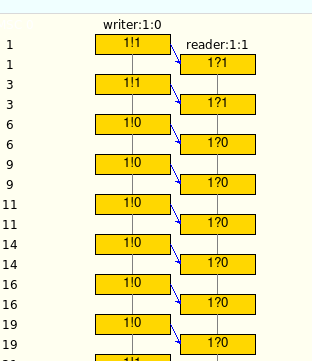
\includegraphics[width=0.3\textwidth]{figures/ex1_simul_example.png}
    }
  \caption{\label{fig:ex1_simulation}A spin simulation of the Promela model from exercise
  1.}
\end{figure}

\newpage

\section*{Exercice 2}

At first, we have implements a \textit{Promela} model that simulate the Wolf,
Sheep and Cabbage problem :

\begin{promelacode}
#define IS_FINISHED (!(present[sheep] && present[cabbage] && present[wolf]))
#define IS_BAD_SITUATION ((present[sheep] && present[cabbage] && !present[wolf]) ||\
                         (present[wolf] && present[sheep] && !present[cabbage]))

/*
  The problem's contraints :
    - the sheep and the wolf can't be left alone
    - the sheep and the cabbage can't be left alone
*/
#define SHEEP_AND_CABBAGE (!(present[sheep] && present[cabbage]))
#define WOLF_AND_SHEEP (!(present[wolf] && present[sheep]))

// To simulate the travel of the boat
#define LEFT 6
#define RIGHT 7

byte turn;

mtype = {wolf, sheep, cabbage};

// to send the item from left to right or right to left
// we could have only 1 channel to simulate this but it is more
// visualable with 2
chan leftToRight = [1] of {mtype};
chan rightToLeft = [1] of {mtype};

proctype leftShore() {
    // initialisation of the leftShore
    bool present[4];
    present[wolf] = true;
    present[sheep] = true;
    present[cabbage] = true;

    // Simulate the travelling of the members
    simulation:
    turn == LEFT;

    // receive the wolf, sheep or cabbage non-derministicly if the item could be acquire with a chanel
    if
        :: rightToLeft?wolf -> present[wolf] = true;
        :: rightToLeft?sheep -> present[sheep] = true;
        :: rightToLeft?cabbage -> present[cabbage] = true;
        :: empty(rightToLeft) -> skip;
    fi

    // send the wolf, sheep or cabbage non-derministicly if the item is present and with
    // respect to the problem's constraints
    
    

    if
        :: present[wolf] && SHEEP_AND_CABBAGE -> leftToRight!wolf; present[wolf] = false;

        :: present[sheep] -> leftToRight!sheep; present[sheep] = false;

        :: present[cabbage] && WOLF_AND_SHEEP -> leftToRight!cabbage; present[cabbage] = false;
    fi

    turn = RIGHT;
    goto simulation;
}

proctype rightShore() {
    // initialisation of the rightShore
    bool present[4];
    present[wolf] = false;
    present[sheep] = false;
    present[cabbage] = false;

    // Simulate the travelling of the members
    simulation:
    turn == RIGHT;

    // receive the item from the boat
    if
        :: leftToRight?wolf -> present[wolf] = true;
        :: leftToRight?sheep -> present[sheep] = true;
        :: leftToRight?cabbage -> present[cabbage] = true;
    fi

    // check is the problem is solved
    if
        :: !(IS_BAD_SITUATION) -> assert(IS_FINISHED);
        :: else -> skip;
    fi

    // eventually send an item back with respect to the problem's constraints
    if
        :: present[wolf] && SHEEP_AND_CABBAGE
        -> rightToLeft!wolf; present[wolf] = false;

        :: present[sheep]
        -> rightToLeft!sheep; present[sheep] = false;

        :: present[cabbage] && WOLF_AND_SHEEP
        -> rightToLeft!cabbage; present[cabbage] = false;

        :: (WOLF_AND_SHEEP) && (SHEEP_AND_CABBAGE)
        -> skip;
    fi

    // pass to the other shore simulation
    turn = LEFT;
    goto simulation;
}

init {
    turn = LEFT; atomic{run leftShore(); run rightShore()};
}
\end{promelacode}

In order to find a solution with \textit{Spin}, we use an assertion on the final
solution :

\begin{promelacode}
#define IS_FINISHED (!(present[sheep] && present[cabbage] && present[wolf]))
#define IS_BAD_SITUATION ((present[sheep] && present[cabbage] && !present[wolf]) ||\
(present[wolf] && present[sheep] && !present[cabbage]))

// check is the problem is solved
if
:: !(IS_BAD_SITUATION) -> assert(IS_FINISHED);
:: else -> skip;
fi
\end{promelacode}

So \textit{Spin} will do his best to find an assertion violation and will
produce the shortest way to violate the assertion which will give us the
optimal solution. The figure~\ref{fig:ex2_simulation} show the \textit{Spin}
simulation that give us the optimal solution to the problem.

\begin{figure}[ht]
  \centering
  \fbox{
    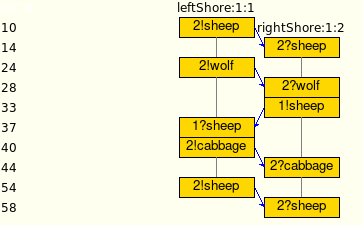
\includegraphics[width=0.4\textwidth]{figures/ex2_shortest_solution.png}
    }
  \caption{\label{fig:ex2_simulation}The shortest solution to the Wolf, Sheep
    and Cabbage problem.}
\end{figure}

Finally, the correct solution is, with the sheep, wolf and cabbage on the left shore :
\begin{enumerate}
\item Send the sheep to the right shore.
\item Go back to the left shore.
\item Send the wolf to the right shore.
\item Send the sheep to the left shore.
\item Send the cabbage to the right shore.
\item Go back to the left shore.
\item Send the sheep to the right shore.
\end{enumerate}

\end{document}

%%% Local Variables:
%%% TeX-command-extra-options: "-shell-escape"
%%% mode: latex
%%% End: